\documentclass{ieeeaccess}
% IEEE Access LaTeX template, version 20260513. The class, fonts and logos are not kept in
% the repository (the fonts are licensed for the template only); put the files of the
% official ACCESS_latex_template zip in template/ before running make.

\usepackage{cite}
\vol{XX}\def\theyear{2026}
\usepackage{amsmath,amssymb}
\usepackage{graphicx}
\usepackage[scaled=0.83]{beramono}
\usepackage{booktabs}
\usepackage{tabularx}
\usepackage{array}
\usepackage{listings}
\usepackage{xcolor}
\usepackage[hyphens]{url}
\usepackage[hidelinks]{hyperref}

\Urlmuskip=0mu plus 0.5mu\relax
\setlength{\emergencystretch}{1.4em}
\newcommand{\code}[1]{{\fontshape{n}\ttfamily #1}}

% Draft markers: numbers that must be regenerated before submission print in red.
\newif\ifdraft \draftfalse
\newcommand{\fresh}[1]{\ifdraft\textcolor{red}{#1}\else #1\fi}
% Every number quoted in the paper, with where it was measured.
% \fresh{...} marks a number that must be regenerated from a committed result before
% submission; it prints in red in draft mode (\drafttrue in main.tex).

% --- Repository designs under the proof (scripts/rtl_prove.sh) -------------------------
% Measured 2026-11-23 at main 00c80f0, Linux x86_64, Z3 from pip (journal entry
% M6.1-rtl-prove-main). 24 testdata/rtl + 18 probes + 8 corpus designs 13..20.
% Re-run 2026-11-23 in the cloud container, release binary at c778e17 (same rtl code as 00c80f0),
% Z3 5.4.1: 45 proved for all runs, 0 bounded; paired registers 0 on 25 designs, at most 9;
% Z3 time for the generated-C++ side 9 to 31 ms per design.
\newcommand{\nDesigns}{50}
\newcommand{\nProved}{45}
\newcommand{\nNotCovered}{5}
\newcommand{\nFailed}{0}
\newcommand{\nBounded}{0}
\newcommand{\nCombinational}{25}
\newcommand{\nMaxPaired}{9}

% --- Mutation check (benchmarks/formal_gate/mutate.py) ---------------------------------
% Run of 2026-11-22 at commit 3c486e4 (journal M6-typed-formal-gates), macOS arm64,
% SystemC 3.0.3, Verilator 5.052. 42 designs given to the script; 40 produced mutants.
% benchmarks/results/formal_gate_mutation_*.json, docs/formal_gates.md.
\newcommand{\nMutDesignsGiven}{42}
\newcommand{\nMutDesigns}{40}
\newcommand{\nMutCompiled}{281}
\newcommand{\nMutSimDiffers}{17}
\newcommand{\nMutProofFinds}{14}
\newcommand{\nMutReaderRejects}{3}
\newcommand{\nMutAccepted}{0}
\newcommand{\nMutSimEqual}{264}
\newcommand{\nMutEqualAccepted}{255}
\newcommand{\nMutEqualRefused}{9}
\newcommand{\nMutNoCompile}{70}
\newcommand{\nMutNoCompileRead}{56}

% --- C2RTL golden models (prove-sec) -----------------------------------------------------
\newcommand{\nGolden}{8}

% --- Stress run on open-source designs (benchmarks/rtl_stress) ---------------------------
% Latest run: journal entry M5.2-clock-gating, 2026-11-23, Linux x86_64, svlang 0.5.1,
% Verilator 5.052, 3,000 steps. The per-design table in benchmarks/results/rtl_stress.md is
% from the earlier run (svlang git 478a0d1) and must be regenerated from the latest run.
\newcommand{\nCodeBases}{16}
\newcommand{\nModules}{2,184}
\newcommand{\nMatch}{1,185}
\newcommand{\nMatchBeforeCG}{1,127}
\newcommand{\nClockRejBefore}{65}
\newcommand{\nClockRejAfter}{13}
% 5 mismatches are from M5.2 (stream_mux, fpnew_cast_multi x2, fpnew_fma_multi x2).
% 994 = 2,184 - 1,185 - 5. The split of the 994 below is from the earlier run (M5.1)
% and sums with the M5.2 figures to 2,183, so it stays red until regenerated.
\newcommand{\nMismatch}{5}
\newcommand{\nRejected}{994}
\newcommand{\nSvlangRej}{\fresh{217}}
\newcommand{\nSvccRej}{\fresh{763}}
\newcommand{\nCrash}{\fresh{13}}
\newcommand{\nPlaceholder}{557}
\newcommand{\nSteps}{3,000}

% --- Comparison with SCAV (benchmarks/scav_compare) --------------------------------------
\newcommand{\nProbes}{18}
\newcommand{\nCorpusRtl}{8}

% --- Size -----------------------------------------------------------------------------
% find crates bindings -name '*.rs' | xargs cat | wc -l at 00c80f0
\newcommand{\nRustLines}{25,700}


\lstset{basicstyle=\ttfamily\scriptsize,columns=fullflexible,keepspaces=true,
  frame=single,framerule=0.3pt,rulecolor=\color{black!40},breaklines=true,
  xleftmargin=2pt,xrightmargin=2pt,aboveskip=4pt,belowskip=4pt}

\hypersetup{
  pdftitle={Translation Validation of SystemVerilog-to-SystemC RTL Conversion by Reading the Generated C++},
  pdfauthor={Mayur Kubavat},
  pdfkeywords={SystemVerilog, SystemC, RTL, translation validation, equivalence checking}
}

\begin{document}
\history{Date of publication xxxx 00, 0000, date of current version xxxx 00, 0000.}
\doi{10.1109/ACCESS.2026.0000000}

\title{Translation Validation of SystemVerilog-to-SystemC RTL Conversion by Reading the Generated C++}

\author{\uppercase{Mayur Kubavat}\authorrefmark{1}}

\address[1]{Independent Researcher, Mountain View, CA 94040, USA}

\tfootnote{This work was done independently, on personal equipment and in a personal capacity. It
is not affiliated with or endorsed by any employer.}

\markboth
{Kubavat: Translation Validation of SystemVerilog-to-SystemC RTL Conversion}
{Kubavat: Translation Validation of SystemVerilog-to-SystemC RTL Conversion}

\corresp{Corresponding author: Mayur Kubavat (e-mail: mkubavat01@gmail.com).}

\begin{abstract}
SystemC models of register-transfer level (RTL) designs are used for virtual platforms, software
bring-up and simulation without a commercial license, and more of them now come from translators
and language models. A wrong model often compiles cleanly: SystemVerilog evaluates an 8-bit sum in
8 bits, while C++ evaluates the same expression in 64, so a missing truncation keeps a carry that
the RTL drops. Our first check of such translations re-read the generated C++ with SystemVerilog's
rules and reported two wrong models as equivalent. This paper describes the check that replaced it
in svcc, an open-source SystemVerilog-to-SystemC converter. The check parses the generated header
with a model of C++17 and SystemC evaluation, turns undefined behavior into proof obligations,
prints the result as SystemVerilog in which every width change is explicit, and proves it
equivalent to a netlist of the source by induction over registers mapped by name. The reference
netlist is built without any svcc code, but both sides use the same SystemVerilog front end. On
\nDesigns{} designs the check proves \nProved{} and reports \nNotCovered{} as outside its model. In
a mutation experiment it accepted none of the \nMutSimDiffers{} mutants that compiled SystemC showed
to be wrong. On \nModules{} modules from \nCodeBases{} open-source code bases, \nMatch{} conversions
match Verilator in random co-simulation, and the check proves \nCorpusProved{} of them equivalent. The runs also found defects in the front end, in svcc and in
Verilator. SystemC process scheduling is checked by co-simulation.
\end{abstract}

\begin{keywords}
Equivalence checking, hardware design languages, RTL, SystemC, SystemVerilog, translation
validation.
\end{keywords}

\titlepgskip=-21pt

\maketitle

\section{Introduction}
\label{sec:intro}

\PARstart{R}{TL} is written in SystemVerilog~\cite{ieee1800_2023}, and much of the work around it runs on
C++ models of the same logic. Virtual platforms boot firmware before silicon, reference models
check RTL in simulation, and SystemC~\cite{ieee1666_2023} models run without a simulator license.
Verilator~\cite{snyder2020verilator} turns RTL into fast C++, and with \code{-{}-sc} into a SystemC
wrapper, but its output is a simulation engine. It is not meant to be read or edited. Readable models come
from hand translation, from translators~\cite{bombieri2010hifsuite,syed2013vhdl2sc,zheng2026bidir}
and from language models asked to translate between C++ and hardware
languages~\cite{collini2024c2hlsc,lyu2026autoc2v}.

None of these sources is verified, and their errors produce no warning. SystemVerilog sizes an
expression from its context. C++ promotes small integer types to \code{int} and converts SystemC's
\code{sc\_uint<W>} to a 64-bit integer. A translation of \code{(a + b) {>}{>} 1} that does not truncate
the sum keeps the carry, and \code{a = b = 0xff} gives \code{0xff} instead of \code{0x7f}. The
two models agree on most inputs.

Translation validation~\cite{pnueli1998tv,necula2000tv,lopes2021alive2} checks each output of a
translator against its input instead of proving the translator correct. Checking C against RTL
with C's own semantics is also old: Clarke, Kroening and Yorav did it with bounded model checking
in 2003~\cite{clarke2003cverilog}, and commercial C-to-RTL equivalence tools do it
today~\cite{koelbl2009c2rtl}. The method in this paper is standard. What we report is what went
wrong when we built the check the obvious way, what we built instead, and how it held up on a
design suite, a mutation experiment and 16 open-source code bases.

The contributions are:
\begin{enumerate}
\item \textbf{A failure report and two design rules.} Our first check re-read the generated C++
with SystemVerilog's rules and reported two wrong models as equivalent. From this we state two
rules for checking any cross-language translator (Section~\ref{sec:failure}).
\item \textbf{The check, \code{svcc rtl-prove}.} It reads the generated header with a model of
C++17 and SystemC evaluation, raises a flag on every operation C++ leaves undefined, and proves the
result equivalent to a netlist of the source by register-mapped induction. Designs outside the
model exit with code 3 (Section~\ref{sec:gate}). The converter it checks is described in
Section~\ref{sec:convert}; a companion software paper covers the tool itself~\cite{kubavat2026svccsx}.
\item \textbf{An evaluation} on \nDesigns{} designs, a mutation experiment judged by compiled
SystemC, \nModules{} modules in co-simulation with Verilator, the proof on the \nMatch{} that
match, the defects these runs found, and a
comparison with a recent translator (Section~\ref{sec:eval}).
\end{enumerate}
\code{svcc} is released under the Apache 2.0 license on crates.io and PyPI, with all scripts and
results.

%% ===========================================================================
\section{Where SystemVerilog and SystemC Differ}
\label{sec:diff}

Table~\ref{tab:diff} lists the rules a translator has to bridge. In each row the same expression
can give different values in the two languages.

\begin{table}[t]
\centering
\caption{Semantic differences between SystemVerilog RTL and SystemC that a translation must bridge.}
\label{tab:diff}
\footnotesize
\setlength{\tabcolsep}{3pt}
\begin{tabularx}{\columnwidth}{@{}>{\raggedright\arraybackslash}p{0.17\columnwidth} >{\raggedright\arraybackslash}X >{\raggedright\arraybackslash}X@{}}
\toprule
Topic & SystemVerilog (IEEE 1800-2023) & C++17 / SystemC \\
\midrule
Width & Context-determined: operands extend to the widest width in the expression and the assignment target (11.6) & Integer promotion to \code{int}; \code{sc\_uint<W>} converts to \code{unsigned long long}; result width set by the C++ type \\
Signedness & Any unsigned operand makes the expression unsigned (11.8) & Usual arithmetic conversions: a mixed comparison is unsigned when the unsigned type's rank is at least the signed type's, or when the signed type cannot hold all its values \\
Undefined ops & Division by zero gives X; shifts beyond the width give 0 & Signed overflow, division by zero and shift $\ge$ width are undefined behavior \\
Update order & Nonblocking updates wait in the nonblocking assignment (NBA) region until all active events of the time step, including a derived clock's change, have run & \code{sc\_signal} updates commit at the end of every delta cycle, so a process woken by a derived clock can see values already updated \\
Values & Four states (0, 1, X, Z) & Two states in \code{sc\_uint}; four in \code{sc\_lv} \\
\bottomrule
\end{tabularx}
\end{table}

A translator that gets every row right still writes C++ that takes a careful reader to check, and
an engineer who knows SystemVerilog tends to read that C++ with SystemVerilog's rules. The first
version of our own check made the same mistake.

%% ===========================================================================
\section{How the First Check Failed}
\label{sec:failure}

\code{svcc} first carried RTL through a text-based path in which expressions were kept as strings
in the intermediate representation (IR). To validate a conversion, the check took the emitted C++,
re-read it as if it were SystemVerilog, and asked a solver whether the re-read design was
equivalent to the source. It reported every design in our suite equivalent.

The comparison with another translator in Section~\ref{sec:scav} needed the generated SystemC to
run on a real SystemC kernel. Two designs the check had proved were wrong
(Table~\ref{tab:fooled}).

\begin{table}[h]
\centering
\caption{Two models the first check reported as equivalent.}
\label{tab:fooled}
\footnotesize
\setlength{\tabcolsep}{3pt}
\begin{tabularx}{\columnwidth}{@{}l >{\raggedright\arraybackslash}X l@{}}
\toprule
Source (8-bit) & What the C++ did & First difference \\
\midrule
\code{y = (a + b) {>}{>} 1} & shifted the 64-bit sum & \code{a=b=0xff}: \code{7f} vs \code{ff} \\
\code{lt = (a - b) < c} & compared the 64-bit difference & \code{a=3e, b=c1, c=7e} \\
\bottomrule
\end{tabularx}
\end{table}

The check could not have found these. Read with SystemVerilog's rules, \code{(a + b) {>}{>} 1}
assigned to an 8-bit target is evaluated in 8 bits, exactly as in the source. The 64-bit
evaluation exists only under C++'s rules, and the check never applied them. The same problem
appears whenever the checked side is derived from the translator's own intermediate form: if the
lowering and the emitter share a misunderstanding, both sides of the comparison inherit it.

Two design rules follow.
\begin{description}
\item[R1] The checked side starts from the emitted header text and gives it the \emph{target}
language's meaning, including the cases the target leaves undefined.
\item[R2] The reference side is built from the source text without any of the translator's code.
\end{description}
R1 and R2 apply to any cross-language translator, including a language model. Our implementation
meets R2 only in part: the reference and the checked side both use the \code{svlang} front end,
which the translator also uses. Section~\ref{sec:assume} treats \code{svlang} as trusted and says
what that costs.

%% ===========================================================================
\section{The Converter}
\label{sec:convert}

\code{svcc rtl2sc} uses \code{svlang}~\cite{kubavat2026svlang}, an open-source SystemVerilog front
end, to parse and elaborate the design. Parameters, \code{localparam}s and generate constructs are
resolved, and every expression is bound with the width and signedness rules of IEEE~1800-2023
clauses 11.6 and 11.8, so each node carries its width and signedness and every implicit
conversion is an explicit node. \code{svcc} lowers this to one typed module per parameter set and
emits one \code{SC\_MODULE} for each.

\emph{Emitter invariant.} Each emitted C++ subexpression evaluates to exactly the value of its
typed node. Wherever C++ would compute in a wider type, the emitter truncates explicitly, so the
8-bit average of Section~\ref{sec:failure} becomes
\begin{lstlisting}[language=C++]
y.write(sc_uint<8>(sc_uint<8>(a.read() + b.read()) >> 1U));
\end{lstlisting}

\emph{Subset.} There is no standard synthesizable subset of SystemVerilog. We follow what
synthesis tools accept~\cite{sutherland2014synth} and stay inside the Accellera synthesizable
subset of SystemC~\cite{ieee1666_1_2016}. Supported constructs are continuous assignments,
\code{always\_comb}, \code{always\_ff} and \code{always\_latch}; blocking and nonblocking
assignment; \code{if}, \code{case}, \code{casez}, \code{casex}, \code{case inside}, \code{for} and
\code{while}; module and package functions; hierarchy with parameter overrides and \code{.*}
connections; bit, part and indexed selects; packed structs, enums and arrays; memories; and vectors
wider than 64 bits (\code{sc\_biguint}). Blocking assignments are read from a local copy inside the
process and written back once. Blocks that drive different bits of one signal are merged into one
process, because a SystemC signal has one writer.

\emph{Clocks.} A register may be clocked by an input, a copy of one, or a register output. A
clock-gating cell (a latch transparent while the clock is low, ANDed with the clock) is converted
to a clock enable on the root clock, and an instance whose clock port is gated gets a module variant
with an enable input. A literal translation would run the gated registers one delta cycle late
(Table~\ref{tab:diff}, update order). The proof does not cover these designs; the evidence for
this conversion is co-simulation (Section~\ref{sec:stress}). Other derived clocks, such as clock
multiplexers, are rejected.

\emph{Fail-closed.} A construct outside the subset is an error with a source location.
\code{svcc} also rejects two things a two-state model would silently read as 0: a signal that is
read but has no driver, and a constant select outside the declared range. X and Z map to 0, which
is the model under which both the proof and the co-simulation run.

%% ===========================================================================
\section{The Check: Reading the Generated C++}
\label{sec:gate}

Fig.~\ref{fig:gate} shows the check. The reference side lowers the source text to a netlist with
\code{svlang} and writes Btor2~\cite{niemetz2018btor2}; no \code{svcc} code runs on that side. The
checked side starts from the generated header.

\begin{figure}[t]
\centering
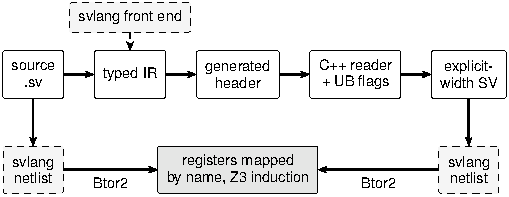
\includegraphics[width=\columnwidth]{fig-gate}
\caption{The \code{rtl-prove} check. The top row up to the header is the translator. The reference
(bottom left) runs no \code{svcc} code. Shaded dashed boxes are \code{svlang}, which all three
paths use and which the check trusts.}
\label{fig:gate}
\end{figure}

\subsection{A model of C++ evaluation}

The reader parses the subset of C++ that \code{rtl2sc} emits and gives each expression the value
C++17 and SystemC give it. \code{bool} and 8- and 16-bit integers promote to \code{int}.
\code{sc\_uint<W>} converts to \code{unsigned long long} and \code{sc\_int<W>} to \code{long long}
(the LP64 data model). Binary operators bring both operands to a common type by the usual arithmetic conversions
and compute in that type. A value is truncated only where the code constructs or assigns a
narrower object. \code{sc\_biguint} arithmetic is exact. A \code{write} in an edge-triggered method
is a nonblocking assignment. A level-sensitive method must be sensitive to every signal it reads;
it is read as combinational logic, or as a latch where it does not assign on every path. Behavior
the standard leaves to the implementation is fixed as C++20 defines it: narrowing to a signed type
wraps, and \code{{>}{>}} of a negative value is arithmetic.

\emph{Undefined behavior.} An operation whose result C++ or SystemC does not define gets no value.
It raises a 1-bit flag, an extra output of the lifted module that the proof must show stays at 0.
The flagged operations are signed overflow, division or modulo by zero, a shift by a negative
amount or by the width or more, a left shift of a negative value, and a select or index out of
range. Guards in the code (\code{?:}, \code{\&\&}, \code{if}) are kept, so a guard the generator
forgot produces a counterexample.

\emph{Explicit-width output.} The reader writes what it computed as SystemVerilog in which every
operator result is self-determined and every width change is a size cast, a concatenation or
\code{\$signed}. SystemVerilog's context sizing therefore cannot change what was read from the C++.
This is the step that closes the gap of Section~\ref{sec:failure}. Internally the reader builds the
same typed design IR that the converter uses and prints it with the same printer; this sharing is
discussed in Section~\ref{sec:assume}.

\subsection{Proof and verdicts}

Both texts are lowered by \code{svlang} to Btor2. Registers are mapped by hierarchical name and
width, one to one, and Z3~\cite{demoura2008z3} checks one inductive step: from any state in which
the mapped registers are equal, the outputs agree, the undefined-behavior flag is 0, and the mapped
registers are equal after a step. If that holds the verdict is \emph{proved}, for every run from
equal start states, with no bound. This is a register-mapped equivalence check; there is no
retiming or state re-encoding. If the inductive step fails, a bounded check from reset (8 steps by
default) gives a concrete \emph{mismatch} or, if none is found, \emph{bounded}. A bounded verdict
is printed as \code{[BND]} and exits with code 2 unless \code{-{}-accept-bounded} is given;
it is not counted as a proof. A register without a partner, or no answer from Z3 on the inductive step, also leads to the bounded check; no answer there is \emph{inconclusive} and counts as a failure. A design
the model does not cover (more than one clock, a multi-dimensional array port, or C++ the reader
does not model) gets \emph{not covered} and exit code 3. The check also proves the lowering (typed
IR against source) separately, which tells a lowering failure apart from an emitter failure.

The same machinery checks an untimed C++ reference function against pipelined RTL with
\code{prove-sec -{}-latency L}: from an arbitrary RTL state, with resets held inactive, the RTL output
equals the function of the inputs $L$ cycles earlier, in the style of C-to-RTL equivalence
checking~\cite{koelbl2009c2rtl}.

\subsection{What a pass assumes}
\label{sec:assume}

A pass holds only under the following assumptions.
(1)~Values are two-state: X and Z read as 0.
(2)~\code{svlang}'s elaboration is taken as the meaning of SystemVerilog. The translator, the
reference and the checked side all use it, so a front-end bug that changes the source's meaning is
invisible to the proof. Three such bugs were found by co-simulation (Section~\ref{sec:defects}),
and the proof could not have found them. The explicit-width text uses only a few plain constructs
to limit this exposure on the checked side.
(3)~There is one clock, and an asynchronous reset takes effect at the clock step.
(4)~The C++ reader is the author's model of C++ typing, not a compiler front end. It was checked
against SystemC~3.0.3 with a probe program and against compiled SystemC by the mutation experiment
of Section~\ref{sec:mutation}. The reader and the converter also share the typed IR and its printer,
so a printer bug could affect both checks.
(5)~Proved means equivalent from equal start states.
(6)~SystemC process scheduling is not modeled. In particular, a process made sensitive to the edge
of an internal copy of a clock is treated as if it were on the root clock. Such a header runs one
delta cycle late in a real kernel and still passes the proof. We confirmed this with a hand-edited
header. Co-simulation is the only check of scheduling.

%% ===========================================================================
\section{Evaluation}
\label{sec:eval}

We ask four questions. \textbf{RQ1}: how much of a design suite does the check prove?
\textbf{RQ2}: does it reject wrong C++, as judged by compiled SystemC? \textbf{RQ3}: how does the
conversion do on real designs, and what defects did those runs find? \textbf{RQ4}: how does
\code{svcc} compare with a recent translator?

\emph{Setup.} \code{svlang}~0.5.1, Z3~5.4.1 (4.15.5 for the corpus proof), Verilator~5.052 and SystemC~3.0.3 (the author's fork of the Accellera
repository, commit \code{9767bff}, C++17). RQ1 was run at \code{svcc} commit \code{00c80f0} on Linux x86\_64
and repeated on the same RTL code in a second Linux container. The mutation experiment (RQ2) was
run at commit \code{5dd247d} on macOS arm64. The stress run (RQ3) was run at commit \code{c8e16fb} and
its proof stage at commit \code{1db5bb2}, both on Linux x86\_64. Every command and result is recorded in the repository's experiment log.

\subsection{RQ1: Proof coverage on the design suite}

The suite has \nDesigns{} designs: 24 construct-group designs in \code{testdata/rtl}, the
\nProbes{} probes of Section~\ref{sec:scav}, and \nCorpusRtl{} pipelined datapaths with C++ golden
models. All are author-written. The check proves \nProved{} by induction, for both the lowering
and the generated C++, and none of these passes is bounded-only. It reports \nNotCovered{} as not
covered: three have more than one clock or a computed clock (\code{clock\_gating},
\code{clock\_vector}, \code{edges\_misc}), one has a multi-dimensional array port
(\code{array\_ports}), and in one the reader does not model a local array copy
(\code{array\_elems}). None fails.

The designs are small. \nCombinational{} of the \nProved{} have no registers to map, so for them
the induction reduces to a combinational equivalence check; the largest has \nMaxPaired{} mapped
registers. Z3 takes 9 to 31~ms per design for the generated-C++ side. All \nGolden{} golden models
prove against their RTL with \code{prove-sec}. One of them, written for an earlier version of this
work, contained undefined behavior (\code{uint16\_t * uint16\_t}, which multiplies in \code{int} and
overflows) that the proof found and that testing with one compiler had not.

\subsection{RQ2: Does the check reject wrong C++?}
\label{sec:mutation}

\emph{Negative tests.} The two designs of Section~\ref{sec:failure} are regression tests that must
fail, together with a dropped sign conversion, an unguarded division, a missing sensitivity entry,
a wrong latency, a datapath bug in RTL, a golden model with promoted-multiply overflow, and C++
outside the subset. All fail.

\emph{Mutation experiment.} Negative tests chosen by the author can share the author's blind
spots, so we compared the proof with an oracle that shares no code with it: compiled SystemC
simulated against Verilator for 5,000 random steps. A script edited the generated header of
\nMutDesignsGiven{} designs one place at a time, changing the width or signedness at which C++
evaluates an expression. \nMutDesigns{} designs produced mutants. Each mutant went to both judges
(Table~\ref{tab:mut}).

\begin{table}[t]
\centering
\caption{Mutation experiment: proof against compiled SystemC co-simulated with Verilator, on mutants of \nMutDesigns{} designs. Edits: (a)~\code{sc\_uint<8>(e)} to \code{(e)}; (b)~to \code{sc\_uint<9>(e)}; (c)~to \code{sc\_int<8>(e)}; (d)~\code{uint64\_t(e)} to \code{(e)}. ``Proof accepts'' counts exit code 0.}
\label{tab:mut}
\footnotesize
\setlength{\tabcolsep}{2.5pt}
\begin{tabular}{@{}l r r r r r@{}}
\toprule
Edit & \shortstack{Com-\\piles} & \shortstack{Sim.\\differs} & \shortstack{Proof\\finds} & \shortstack{Reader\\rejects} & \shortstack{Proof\\accepts} \\
\midrule
drop truncation (a) & 133 & 7 & 4 & 3 & 0 \\
one bit wider (b) & 106 & 5 & 5 & 0 & 0 \\
flip signedness (c) & 28 & 5 & 5 & 0 & 0 \\
drop built-in cast (d) & 14 & 0 & 0 & 0 & 0 \\
\midrule
Total & \nMutCompiled{} & \nMutSimDiffers{} & \nMutProofFinds{} & \nMutReaderRejects{} & \textbf{\nMutAccepted{}} \\
\bottomrule
\end{tabular}
\end{table}

No mutant that the simulation showed to be wrong was accepted: \nMutProofFinds{} produced a
counterexample and \nMutReaderRejects{} were refused by the reader. Of the \nMutSimEqual{} mutants
that simulate equal, the proof accepted \nMutEqualAccepted{} and the reader refused
\nMutEqualRefused{}. The proof never reported a difference that the simulation did not see. Most
edits are harmless because an outer construction truncates again, so only \nMutSimDiffers{}
mutants change behavior, in 10 designs. The experiment does not tell bounded from inductive passes
apart, and it was run at an earlier commit than RQ1.

The experiment has clear limits. All four edits touch casts, the class of error R1 was built for.
There are no mutations of sensitivity lists, edge kinds, process sensitivity on internal signals,
operators, constants or indices; assumption (6) says at least one of these would be accepted. A
further \nMutNoCompile{} mutants did not compile, and the reader accepted \nMutNoCompileRead{} of
them, because it is not a type checker. \code{rtl-prove} does not compile the header itself;
co-simulation does. The result is evidence that the C++ model agrees with real SystemC on cast
and width edits in small designs. The paper does not claim more than that.

\subsection{RQ3: Real designs}
\label{sec:stress}

We tried every module of \nCodeBases{} open-source code bases as a top with its default
parameters: picorv32, SERV, biRISC-V, verilog-axi, SCR1, tech\_cells\_generic, common\_cells,
PULP AXI, CVFPU, Ibex, CV32E40P, CV32E40X, CVA6, Caliptra, OpenTitan and BaseJump STL, \nModules{}
modules in all. Each module passes through three stages: convert, compile the header against
SystemC, and co-simulate against Verilator for \nSteps{} random steps, comparing every output after
every step. Each step changes the data inputs and then toggles one clock chosen at random, so a run has
1,500 clock cycles in all, about $1{,}500/k$ per clock for a module with $k$ clocks. Both models run two-state, inputs that reach an edge
sensitivity are driven as clocks one at a time, synchronous resets are ordinary random inputs, and
Verilator is built without the \code{VERILATOR} macro so that both models come from the same text.
No coverage was measured.

\nMatch{} modules convert, compile and match Verilator, and \nMismatch{} differ. The other
\nRejected{} are rejected by the front end or by \code{svcc} with a located error, or exceed 2~GB or
120~s. Many rejections are not real gaps: a module tried alone with placeholder defaults
(\code{parameter type T = logic}, a width of 0 or $-1$, an unconnected interface port) is not a valid
top, and the \code{svlang} front-end test corpus classifies \nPlaceholder{} such modules. The
largest genuine gaps are unpacked structs and struct-typed ports through type parameters,
interfaces, hierarchical references, and array ports connected to anything but a whole array.
Coverage is uneven across code bases: most of CVA6 and PULP AXI is rejected, and most matching
modules are leaf cells or blocks, not whole cores.

Converting clock-gating cells to enables (Section~\ref{sec:convert}) moved the result from
\nMatchBeforeCG{} to \nMatch{} matching modules and cut clock-related rejections from
\nClockRejBefore{} to \nClockRejAfter{}, with no module going from match to mismatch. Of the
\nMismatch{} remaining differences, none is an \code{svcc} defect. One is a Verilator defect: in
a module with a placeholder parameter, an out-of-range write lands on an in-range bit. The two in
CVFPU's cast unit, and the first difference in its fused multiply-add, come from a front-end width
error on \code{**} in a sized parameter, fixed by an unreleased \code{svlang} change (commit
\code{af574c9}). With that fix, the fused multiply-add differs only when the random format code
names no format. The module then reads its per-format arrays out of range, so the result is x
under clause~11.5.1 of IEEE~1800-2023. With the format inputs limited to valid codes, the two
models agree for 200,000 steps.

\emph{Proof on the matching modules.} \code{rtl-prove} accepts multi-file designs, so the check was
run on every module that matched Verilator, \nProofRecords{} records counting a module once per
code base. It proved \nCorpusProved{}, gave a bounded-only result for \nCorpusBounded{}, failed on
\nCorpusFail{} and reported \nCorpusNotCovered{} as outside its model, with no tool errors. Of the
proved modules, \nCorpusComb{} have no registers; the largest has \nCorpusMaxRegs{} mapped
registers, and Z3 took a median of 28~ms and at most 44~s per module. None of the failures is a
functional difference. In \nCorpusUnknown{} Z3 returned no answer, \nCorpusUnsupported{} use a
construct the reader rejects (eight are clock-gating latches written with a nonblocking
assignment), \nCorpusNoOutputs{} have no outputs to compare, and \nCorpusFalseDiff{} are false
differences caused by the check's start-state constraint on \code{integer} loop variables that the
front end infers as latches. Most modules outside the model have more than one clock or use
assertions with \code{\$isunknown}. Bounded-only results are not counted as proofs.

\emph{Defects found.}
\label{sec:defects}
Running one design through \code{svlang}, \code{svcc}, a SystemC kernel and Verilator and comparing
the results is a differential test of those tools, as done for C
compilers~\cite{yang2011csmith} and synthesis tools~\cite{herklotz2020verismith}. Each defect
below gave a wrong result with no diagnostic.

\code{svcc}: (1)~A process holding a local copy of an array wrote every element back, including
elements driven by other processes, which lost updates or caused a multiple-driver abort. (2)~A
wildcard \code{.*} connection bound only its first port; this alone accounted for 57 mismatching
Caliptra modules. (3)~A register clocked by a plain copy of the clock (\code{assign gclk = clk}) ran
one delta cycle late. Registers behind clock-gating cells did the same; that was already a known
limit and led to the conversion of Section~\ref{sec:convert}. Each case now has a regression design.
Defect (3) is a scheduling effect, which co-simulation checks (assumption (6)).

\code{svlang}: three elaboration defects, confirmed against IEEE~1800-2023 and fixed in
\code{svlang}~0.5.1. A generate \code{if} on a reduction of a parameter elaborated neither branch;
a fill literal \code{'1} as a sized parameter default evaluated to 1; and a select on a struct member
with its own range was bound against the wrong range. They change the netlist that every user of
that front end sees.

Verilator: (1)~a module that instantiates itself is built without its children when it is
selected with \code{-{}-top-module}, and its output stays 0. Here the reference was wrong and
\code{svcc} was right; \code{rtl-cosim} now wraps such a top. (2)~An out-of-range write through a
variable select changes an in-range bit when the vector has a negative bound, as in
\code{[-1:0]}, or when the index selects past a packed two-dimensional array whose size is not a
power of two. Clause~11.5.1 says such a write has no effect. Both are present in 5.020 and in the
development version (5.055, commit \code{a53cbcd}), and Icarus Verilog~12 gives the expected
result. They are reported as Verilator issues 9328 and 9329~\cite{verilator9328,verilator9329}.

\subsection{RQ4: Comparison with a recent translator}
\label{sec:scav}

Zheng et al.~\cite{zheng2026bidir} present a bidirectional translator between SystemC and Verilog.
We compare with SCAV, a public implementation of that translator (commit \code{2ef2e6b}). Its
Verilog-to-SystemC direction rewrites a text dump of a Verilog-2005 parse tree with regular
expressions, and its SystemC-to-Verilog direction recognizes the method names its own forward
direction generates. It does not check its output. We have not reproduced the article's own
evaluation.

We used two inputs: the \nCorpusRtl{} pipelined datapaths of RQ1, and \nProbes{} probes written
for this study, each targeting one construct (blocking assignments in combinational and sequential
blocks, signed arithmetic, parameters, wide vectors, memories, loops, \code{casez}, functions,
generate, part selects, a state machine, hierarchy, counters, the width rule, wrap-around, and
latch ordering). A result counts as correct if the output compiles against SystemC and matches the
source in co-simulation. SCAV's translator stopped with an internal error on 3 of the
\nCorpusRtl{} datapaths and 9 of the \nProbes{} probes. Its output compiled for 0 of the datapaths
and 2 of the probes, and was correct for none. Of the 9 examples shipped with SCAV, 3 compiled and 1
of those simulated wrongly. SCAV was judged against Icarus Verilog with SystemC 2.3.4.

\code{svcc} is correct on all \nCorpusRtl{} datapaths and all \nProbes{} probes, judged with
\code{rtl-cosim} against Verilator with SystemC 3.0.3, and the check proves them. The two tools were
therefore run under different harnesses. The probes are also part of \code{svcc}'s own suite and
were used during its development: the same probes run against \code{svcc}'s earlier text-based path
gave 3 of \nProbes{}, and that result is what exposed the failure of Section~\ref{sec:failure}. The
comparison shows that SCAV does not handle these constructs. It is not a benchmark on neutral
ground.

%% ===========================================================================
\section{Related Work}
\label{sec:related}

\emph{Hardware description language (HDL) to SystemC translation.} HIFSuite~\cite{bombieri2010hifsuite} converts VHDL and Verilog
to SystemC and back through a common intermediate format, and Syed et al.~\cite{syed2013vhdl2sc}
translate RTL VHDL to SystemC with attention to process and delta-cycle mapping.
v2c~\cite{mukherjee2016v2c} translates synthesizable Verilog to C so that software verifiers can
check RTL. Zheng et al.~\cite{zheng2026bidir} translate in both directions between SystemC and
Verilog. Verilator~\cite{snyder2020verilator} produces SystemC for simulation.

\emph{C and RTL consistency.} Clarke, Kroening and Yorav check a C program against Verilog by
unrolling both under their own semantics~\cite{clarke2003cverilog}, the approach behind
hw-cbmc and later C-to-RTL tools; CBMC~\cite{clarke2004cbmc} gives the
bit-precise C semantics. Word-level sequential equivalence between C/C++ models and
RTL~\cite{koelbl2009c2rtl} is supported by commercial tools. R1 is the premise of all of this
work. \code{rtl-prove} applies it to the output of a translator, with a C++ model limited to the
code that translator emits, and \code{prove-sec} is a small open version of C-to-RTL checking.
Yosys EQY~\cite{yosys_eqy} checks equivalence between two RTL or netlist versions.

\emph{Translation validation and verified compilation.} Translation validation was proposed by
Pnueli et al.~\cite{pnueli1998tv}, applied to a production compiler by Necula~\cite{necula2000tv}
and to LLVM by Alive2~\cite{lopes2021alive2}, whose treatment of undefined behavior we follow. In
hardware, Kundu et al.~\cite{kundu2010tvhls} validate high-level synthesis with a simulation
relation that need not be a one-to-one register map, which is more general than our name-based
mapping. The alternative is a verified
translator: CompCert~\cite{leroy2009compcert} for C, Vericert~\cite{herklotz2021vericert} for C to
Verilog, and Lutsig~\cite{loow2021lutsig} for a Verilog subset to netlists. These give stronger
guarantees over smaller subsets.

\emph{Semantics.} Müller et al.~\cite{mueller2001scsem} give a formal simulation semantics of
SystemC, and Herber et al.~\cite{herber2008scta} model check SystemC designs, including the
scheduler, with timed automata; our proof does not model the scheduler at all.

\emph{Language models.} Language models generate Verilog~\cite{liu2023verilogeval} and
translate C++ to high-level-synthesis-ready code or Verilog~\cite{collini2024c2hlsc,lyu2026autoc2v}. Their outputs
are mostly judged by tests. A check
that reads generated code with the target's semantics can judge such outputs too, provided they
stay inside the subset the reader models. We have not evaluated this.

%% ===========================================================================
\section{Scope}
\label{sec:limits}

The proof's guarantee holds under the assumptions of Section~\ref{sec:assume}. In practice:

\begin{itemize}
\item Proofs cover single-clock designs with two-state values, with asynchronous reset applied at
the clock step. Multi-clock and X-dependent behavior, and SystemC process scheduling, are covered
by co-simulation against Verilator on a real SystemC kernel.
\item A bounded verdict is reported separately, exits with code 2, and is not counted as a proof.
\item The testbench direction of \code{svcc} (UVM-SystemC, CRAVE and FC4SC) is outside this paper.
\end{itemize}

%% ===========================================================================
\section{Conclusion}
\label{sec:conclusion}

Our first check for a SystemVerilog-to-SystemC translator used SystemVerilog's semantics on the
C++ output and passed wrong models. Reading the generated C++ with C++'s rules, flagging undefined
behavior and proving against a netlist of the source closed that gap on the designs we tried, and a
mutation experiment against compiled SystemC found no cast or width error the check accepted. The
check leaves scheduling to co-simulation and reports bounded verdicts separately. On real code the converter
produces \nMatch{} modules that match Verilator, \nCorpusProved{} of which the check proves
equivalent, and the same runs found defects in three tools. Next steps are a scheduling check for
processes on internal clocks, multi-clock designs, a separate verdict for solver unknowns, and the
same treatment for the testbench direction.

%% ===========================================================================
\section*{Data and Code Availability}

\code{svcc} (Rust, \nRustLines{} lines, with Python bindings), the design suite, the probes, the
mutation and stress scripts, and all results are at \url{https://github.com/mayurkubavat/svcc}
under the Apache 2.0 license. Every release is archived on Zenodo~\cite{kubavat2026svcczenodo}. Each measurement in this paper is recorded with
its command, commit, machine and tool versions in the repository's experiment log
(\code{results/experiment\_log.jsonl}).

\section*{Acknowledgment}

This work received no external funding, and the author declares no conflict of interest. The author thanks the maintainers of Verilator, SystemC and Z3. The author used Google Antigravity
IDE to help develop the \code{svcc} implementation and to refine this manuscript, and other AI coding
and writing assistants to help prepare parts of the benchmark scripts, the evaluation runs and the
manuscript text. The author
reviewed all of it, ran and checked every measurement, proof and reference reported here, and takes
full responsibility for the content.

\bibliographystyle{IEEEtran}
\bibliography{refs}

\begin{IEEEbiography}[{\includegraphics[width=1in,height=1.25in,clip,keepaspectratio]{photo-kubavat.jpg}}]{Mayur Kubavat}
received the M.E. degree in VLSI and Embedded Systems Design from Gujarat Technological
University, Ahmedabad, India, in 2015.

He has worked in ASIC and SoC Design Verification since 2016, including at Google, in Bangalore,
India, and in Mountain View and Sunnyvale, CA, USA, from 2019 to 2026, on processor and accelerator
designs. He is currently a Design Verification Engineer in industry. His research interests
include Hardware Verification, SystemVerilog, SystemC, Formal Methods, and open-source Electronic
Design Automation (EDA) tools.
\end{IEEEbiography}

\EOD

\end{document}
